Snapshotting is een vorm van on-site backup. Een bestandssysteem werkt met pointers naar de data. Een snapshot deze nieuwe pointers naar de data. De data op disk en de data op de snapshot is dus hetzelfde. Als een bestand gewijzigd wordt dan veranderd op het bestandssysteem de pointer naar de nieuwe data, terwijl de pointer vanuit de snapshot blijft staan naar de oude data. Zie figuur \ref{fig:snapshot} voor een grafische weergave van de werking van snapshots.

\begin{figure}[h]
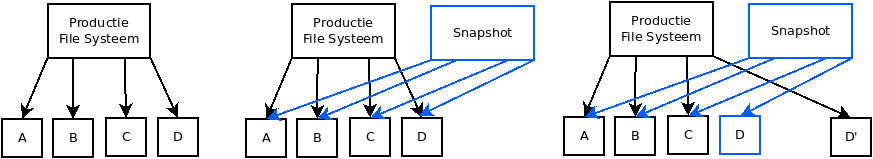
\includegraphics[width=\textwidth]{snapshot}
\centering
	\caption{Hoe snapshotting werkt}
	\label{fig:snapshot}
\end{figure}

